\documentclass[border=4pt,tikz]{standalone}
\usepackage[T1]{fontenc}
\usepackage{lmodern}
\usepackage{amsmath}
\usetikzlibrary{positioning,arrows.meta,calc,fit,backgrounds,patterns}
% Shared visual language for the paper's architecture diagrams.
% Every fill differs in lightness, so the diagrams stay legible when printed
% in grayscale; colour is only a redundant cue.
\definecolor{ink}{HTML}{1B2A3A}
\definecolor{navyfill}{HTML}{D5E0EC}
\definecolor{navyedge}{HTML}{2F5D8A}
\definecolor{tealfill}{HTML}{BFD8D5}
\definecolor{tealedge}{HTML}{2A6F6C}
\definecolor{amberfill}{HTML}{F1DCAE}
\definecolor{amberedge}{HTML}{9C6512}
\definecolor{greyfill}{HTML}{E5E7EB}
\definecolor{greymid}{HTML}{8B939E}
\definecolor{redfill}{HTML}{F0CBC5}
\definecolor{rededge}{HTML}{9E3B32}

\tikzset{
  >={Stealth[length=2.0mm,width=1.5mm]},
  every node/.style={font=\footnotesize, text=ink},
  box/.style={draw=ink, line width=0.5pt, rounded corners=1.5pt,
              fill=greyfill, align=center, inner sep=3pt, minimum height=7mm},
  databox/.style={box, fill=amberfill, draw=amberedge},
  procbox/.style={box, fill=navyfill, draw=navyedge},
  repbox/.style={box, fill=tealfill, draw=tealedge},
  evalbox/.style={box, fill=redfill, draw=rededge},
  fadebox/.style={box, fill=white, draw=greymid, dashed},
  arr/.style={->, draw=ink, line width=0.6pt},
  darr/.style={->, draw=greymid, line width=0.6pt, dashed},
  lbl/.style={font=\scriptsize, text=ink, inner sep=1pt, fill=white, fill opacity=0.85, text opacity=1},
  note/.style={font=\scriptsize, text=ink, align=left, inner sep=1pt},
  badge/.style={draw=rededge, fill=redfill, rounded corners=6pt,
                font=\scriptsize\bfseries, text=rededge, inner sep=2.2pt},
  badgefrz/.style={draw=tealedge, fill=tealfill, rounded corners=6pt,
                font=\scriptsize\bfseries, text=tealedge, inner sep=2.2pt},
  group/.style={draw=greymid, line width=0.5pt, rounded corners=3pt, inner sep=6pt},
}


\newcommand{\head}[2]{%
  \draw[draw=ink, line width=0.6pt, fill=greyfill] (#1,#2) circle (0.46);
  \fill[ink] (#1-0.16,#2+0.10) circle (0.035);
  \fill[ink] (#1+0.16,#2+0.10) circle (0.035);
  \draw[draw=ink, line width=0.5pt] (#1,#2+0.05) -- (#1,#2-0.10);
  \draw[draw=ink, line width=0.5pt] (#1-0.15,#2-0.26) -- (#1+0.15,#2-0.26);
}
\newcommand{\phone}[1]{%
  \draw[draw=amberedge, fill=amberfill, line width=0.5pt, rounded corners=1pt]
        ([xshift=-0.13cm,yshift=-0.22cm]#1) rectangle ([xshift=0.13cm,yshift=0.22cm]#1);
}
\newcommand{\lamp}[1]{%
  \draw[draw=ink, fill=amberfill, line width=0.5pt] (#1) circle (0.16);
  \foreach \a in {0,45,90,135,180,225,270,315}
    \draw[draw=ink, line width=0.4pt] (#1) ++(\a:0.22) -- ++(\a:0.10);
}
\newcommand{\nocapture}[2]{%
  \head{#1}{#2};
  \draw[draw=rededge, line width=1.1pt] (#1-0.42,#2-0.42) -- (#1+0.42,#2+0.42);
  \draw[draw=rededge, line width=1.1pt] (#1-0.42,#2+0.42) -- (#1+0.42,#2-0.42);
  \node[font=\scriptsize\bfseries, text=rededge, anchor=north] at (#1,#2-0.62) {not captured};
}

\begin{document}
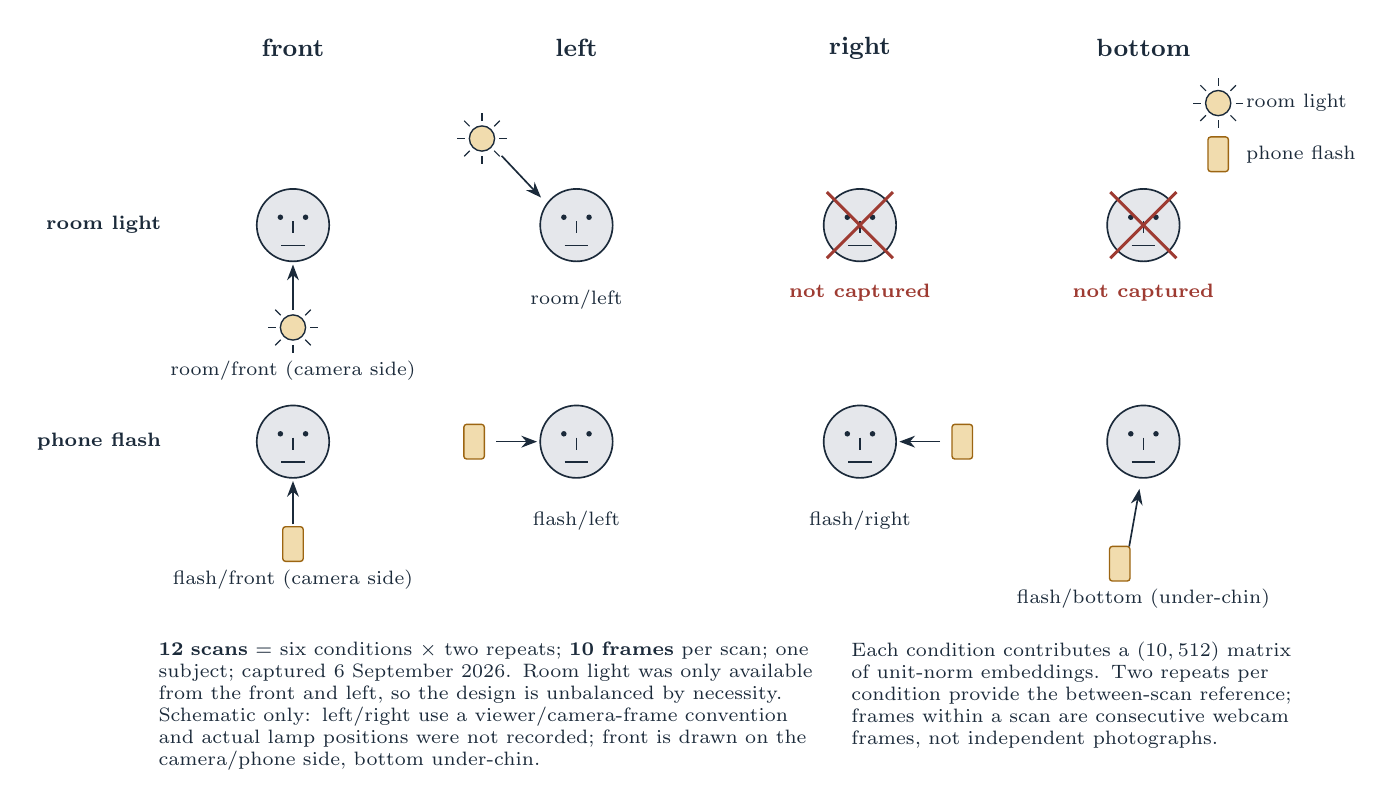
\begin{tikzpicture}[x=1cm,y=1cm]

% ---------------------------------------------------------------- column labels
\node[font=\small\bfseries, text=ink] at (1.80,5.55) {front};
\node[font=\small\bfseries, text=ink] at (5.40,5.55) {left};
\node[font=\small\bfseries, text=ink] at (9.00,5.55) {right};
\node[font=\small\bfseries, text=ink] at (12.60,5.55) {bottom};

% ---------------------------------------------------------------- room row
\node[font=\scriptsize\bfseries, text=ink, anchor=east] at (0.25,3.30) {room light};
\head{1.80}{3.30}
  \lamp{1.80,2.00}
  \draw[arr] (1.80,2.28) -- (1.80,2.80);
  \node[font=\scriptsize, anchor=north] at (1.80,1.70) {room/front (camera side)};

\head{5.40}{3.30}
  \lamp{4.20,4.40}
  \draw[arr] (4.45,4.18) -- (4.95,3.65);
  \node[font=\scriptsize, anchor=north] at (5.40,2.60) {room/left};
\nocapture{9.00}{3.30}
\nocapture{12.60}{3.30}

% ---------------------------------------------------------------- flash row
\node[font=\scriptsize\bfseries, text=ink, anchor=east] at (0.25,0.55) {phone flash};

\head{1.80}{0.55}
  \phone{1.80,-0.75}
  \draw[arr] (1.80,-0.50) -- (1.80,0.05);
  \node[font=\scriptsize, anchor=north] at (1.80,-0.95) {flash/front (camera side)};

\head{5.40}{0.55}
  \phone{4.10,0.55}
  \draw[arr] (4.38,0.55) -- (4.90,0.55);
  \node[font=\scriptsize, anchor=north] at (5.40,-0.20) {flash/left};

\head{9.00}{0.55}
  \phone{10.30,0.55}
  \draw[arr] (10.02,0.55) -- (9.50,0.55);
  \node[font=\scriptsize, anchor=north] at (9.00,-0.20) {flash/right};

\head{12.60}{0.55}
  \phone{12.30,-1.00}
  \draw[arr] (12.42,-0.78) -- (12.55,-0.05);
  \node[font=\scriptsize, anchor=north] at (12.60,-1.20) {flash/bottom (under-chin)};

% ---------------------------------------------------------------- source legend
\lamp{13.55,4.85}
\node[font=\scriptsize, anchor=west] at (13.78,4.85) {room light};
\phone{13.55,4.20}
\node[font=\scriptsize, anchor=west] at (13.78,4.20) {phone flash};

% ---------------------------------------------------------------- design facts
\node[note, anchor=north west, text width=8.4cm] at (0.05,-1.95)
  {\textbf{12 scans} $=$ six conditions $\times$ two repeats; \textbf{10 frames} per scan;
   one subject; captured 6 September 2026. Room light was only available from the front and left,
   so the design is unbalanced by necessity. Schematic only: left/right use a viewer/camera-frame convention and actual lamp
   positions were not recorded; front is drawn on the camera/phone side, bottom under-chin.};
\node[note, anchor=north west, text width=5.6cm] at (8.85,-1.95)
  {Each condition contributes a $(10,512)$ matrix of unit-norm embeddings. Two repeats per
   condition provide the between-scan reference; frames within a scan are consecutive webcam
   frames, not independent photographs.};

\end{tikzpicture}
\end{document}
